\documentclass[a4paper,12pt]{article}
\usepackage[utf8]{inputenc}
\usepackage[russian]{babel}
\usepackage{graphicx}
\usepackage{geometry}
\geometry{left=2cm,right=2cm,top=2cm,bottom=2cm}
\usepackage{amsmath}
\usepackage{hyperref}
\usepackage{makecell}

\title{Влияние графовых представлений на коллективное рассуждение LLM-агентов в игре «Мафия»}
\author{Пеганов Никита, Назарько Михаил}
\date{2025}

\begin{document}

\maketitle

\begin{abstract}
В работе исследуется влияние включения графовых представлений отношений между игроками на успешность коллективных рассуждений LLM-агентов в игре «Мафия». Мы сравниваем различные схемы инъекции графа в промпт и фиксируем статистику побед для разных режимов и LLM-моделей. Результаты свидетельствуют о выигрыше стратегий с графом, основанным на накопленной истории взаимодействий.
\end{abstract}

\section{Введение}
Современные языковые модели (LLM) демонстрируют способность к рассуждению и коллективному мышлению в игровых и социальных задачах. Одна из ключевых проблем — сохранение и использование сложного контекста взаимодействий. Мы выдвигаем гипотезу, что графовое представление отношений между игроками, построенное из истории обсуждений, может существенно повысить эффективность кооперации и качество принятых решений в полукооперативных играх, таких как «Мафия».

\section{Методология}
Проект основан на форке репозитория \texttt{llm-mafia-game}, адаптированного для запуска с локальными моделями (vllm). Все агенты в эксперименте — клоны одной LLM. Эксперименты симулируются батчами по 80 партий на различных моделях и с разными видами графовых подсказок. Используется автоматизированная система логирования и сбора результатов на платформе Firebase, а для анализа предусмотрен веб-дэшборд.

\begin{figure}[h!]
    \centering
    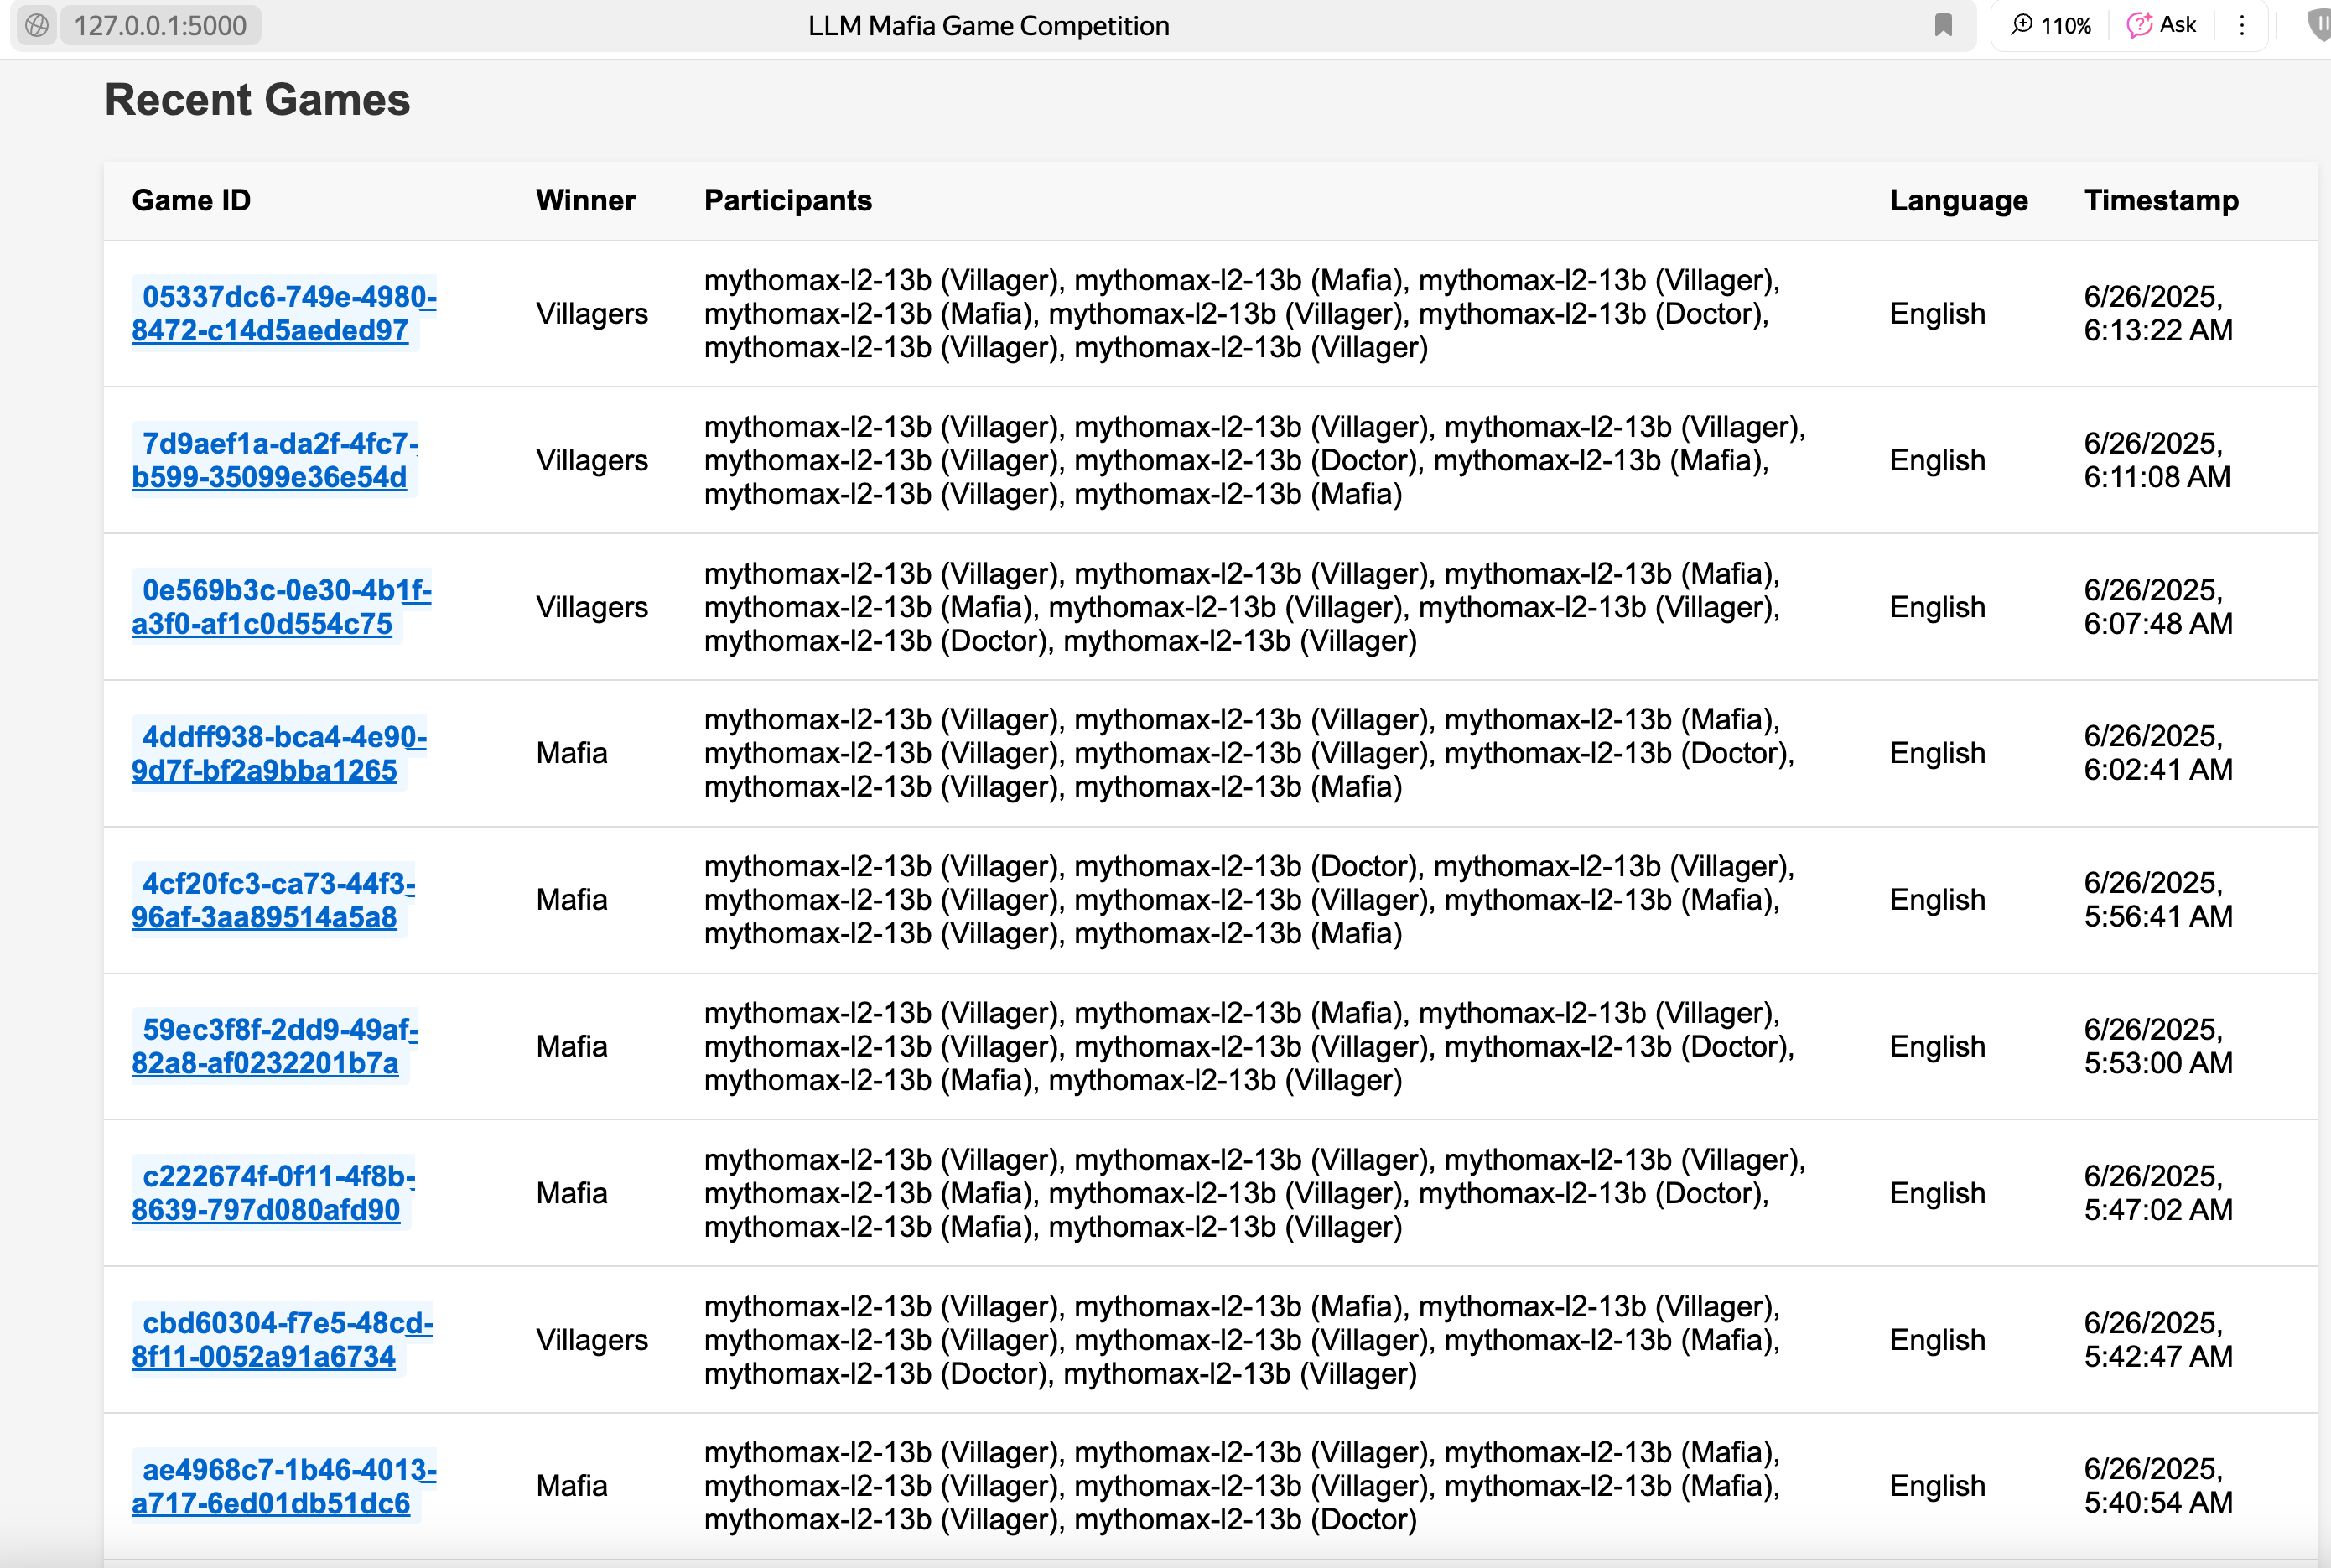
\includegraphics[width=0.85\linewidth]{dashboard.png}
    \caption{Веб-дэшборд для мониторинга партий, статистики и истории}
    \label{fig:dashboard}
\end{figure}

\section{Модели и алгоритмы}
Для экспериментов использовались различные open-source LLM: \texttt{gryphe/mythomax-l2-13b}, \texttt{mistralai/mistral-small-24b-instruct-2501}, \texttt{deepseek/deepseek-llm-7b-chat} и др. Графы строит отдельная аналитическая LLM, анализируя диалоги и действия игроков. Рассматривались следующие типы графов:

\begin{itemize}
    \item \textbf{Коммуникационный граф} — связи между игроками на основе явных взаимодействий (обвинения, защита, голосования)
    \item \textbf{Граф текущего раунда} — только связи в рамках одного круга
    \item \textbf{Глобальный граф} — агрегация всей истории взаимодействий и событий
\end{itemize}

\begin{figure}[h!]
    \centering
    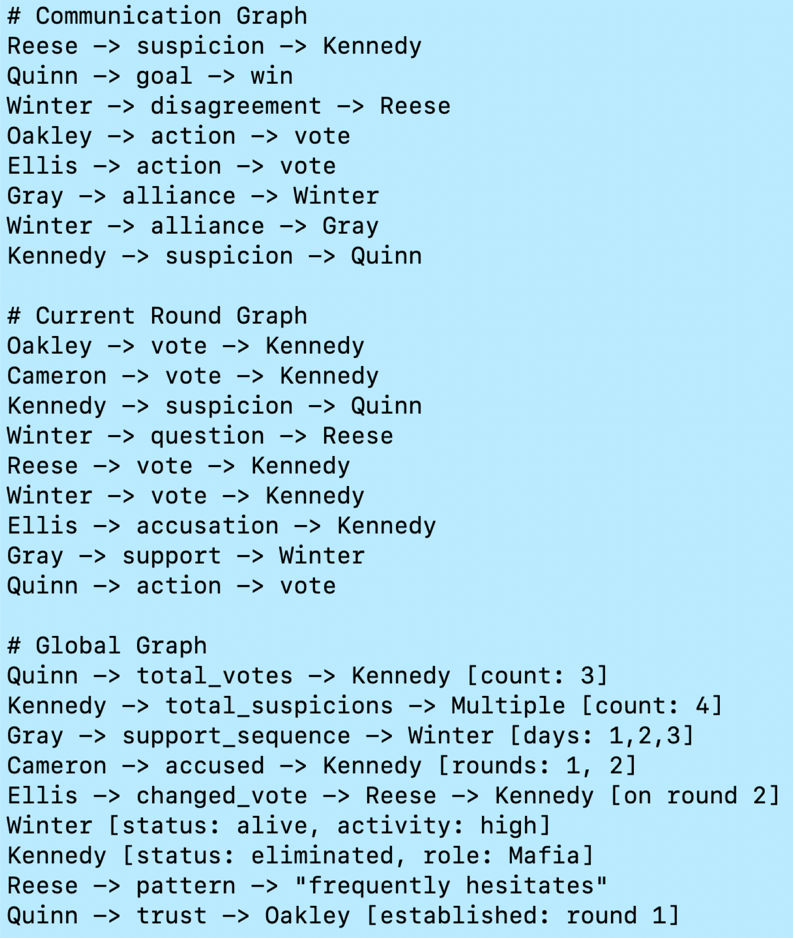
\includegraphics[width=0.6\linewidth]{graph_types.png}
    \caption{Примеры различных типов графов в игре}
    \label{fig:graphs}
\end{figure}

\section{Результаты}

\begin{figure}[h!]
    \centering
    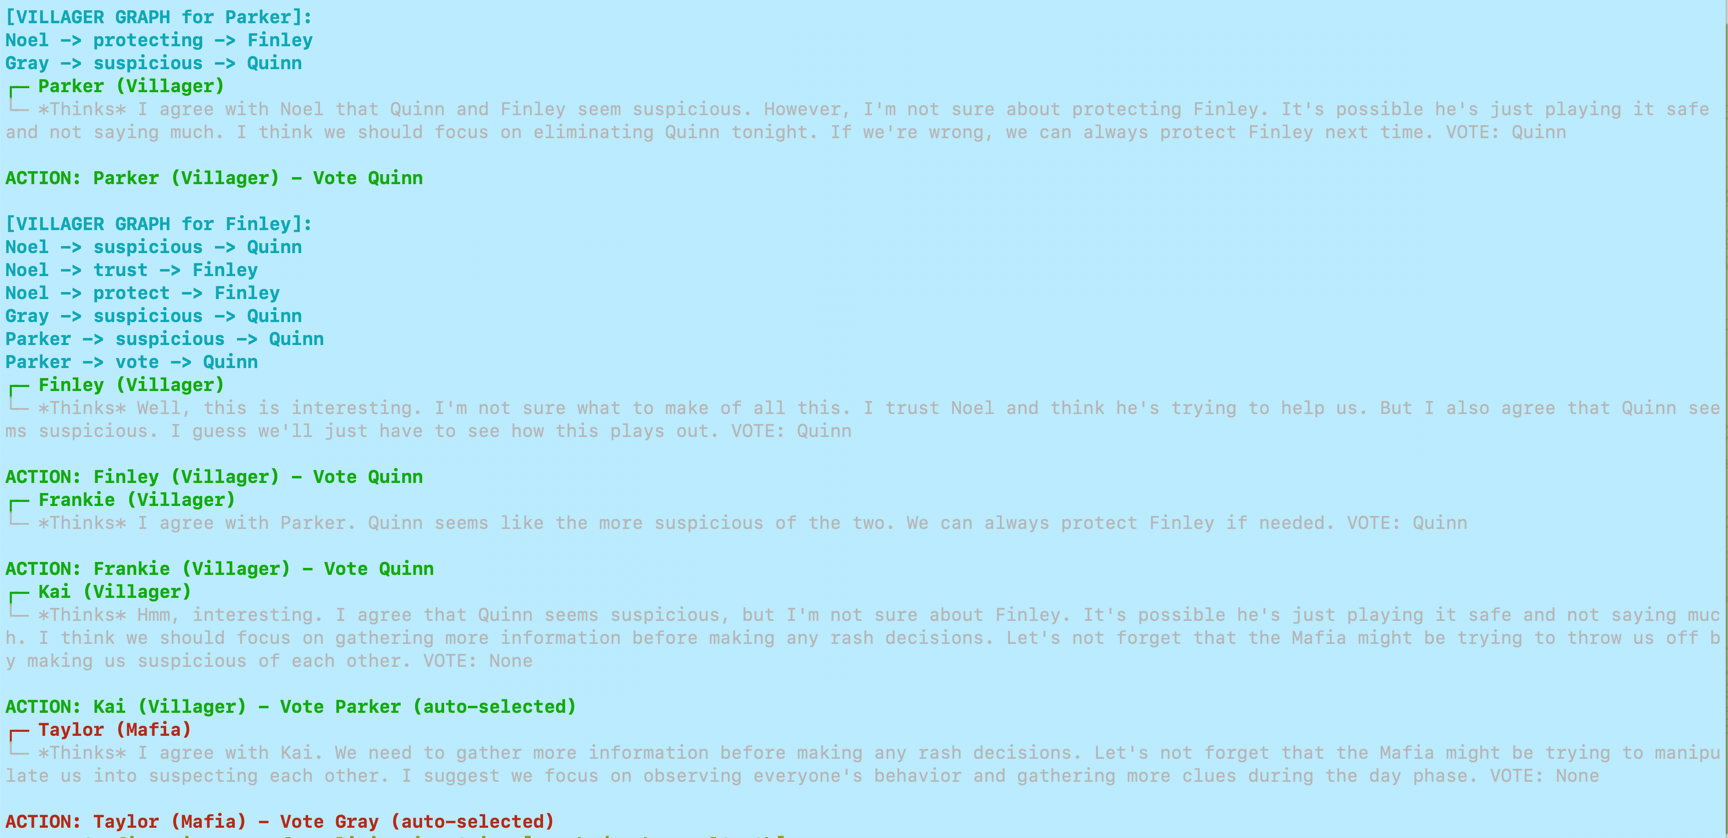
\includegraphics[width=0.8\linewidth]{demonstration.png}
    \caption{Демонстрация графа отношений, внедрённого в промпт для LLM-агента}
    \label{fig:demo}
\end{figure}

Таблица \ref{tab:results} демонстрирует число побед мирных игроков (из 80 партий) для разных моделей и режимов графовой инъекции:

\begin{table}[h!]
\centering
\renewcommand{\arraystretch}{1.2}
\begin{tabular}{|l|c|c|c|c|c|c|}
\hline
\textbf{Модель} &
\makecell{\textbf{Без}\\\textbf{графа}} &
\makecell{\textbf{Ком-}\\\textbf{муник.}} &
\makecell{\textbf{Комм.}\\\textbf{история}} &
\makecell{\textbf{Раунд}} &
\makecell{\textbf{Раунд}\\\textbf{история}} &
\makecell{\textbf{Глобал.}\\\textbf{история}} \\
\hline
mythomax-l2-13b & 41 & 37 & 48 & 39 & 50 & 55 \\
mistral-small-24b-instruct-2501 & 39 & 36 & 47 & 38 & 49 & 56 \\
deepseek-llm-7b-chat & 40 & 35 & 45 & 38 & 47 & 54 \\
deepseek-r1-distill-llama-70b & 42 & 38 & 49 & 39 & 51 & 58 \\
hermes-3-llama-3.1-70b & 41 & 36 & 46 & 40 & 48 & 55 \\
DeepSeek-R1-Distill-Qwen-32B & 40 & 35 & 46 & 39 & 48 & 54 \\
\hline
\end{tabular}
\caption{Число побед мирных игроков из 80 партий для разных моделей и режимов графов}
\label{tab:results}
\end{table}

\section{Обсуждение}
Результаты показали, что графы без накопления истории малоэффективны: агенты теряют контекст и не могут скоординировать действия. Наилучших результатов удалось достичь при использовании общего глобального графа с накоплением истории — winrate мирных превышает случайный. Граф текущего раунда показал минимальное влияние. Повторение экспериментов автора на локальных моделях подтверждает воспроизводимость подхода и даёт простор для масштабных исследований.

\section{Заключение}
Включение графовых представлений, особенно основанных на всей истории игры, позволяет языковым моделям эффективнее коллективно рассуждать и добиваться более высоких победных стратегий в социальных играх. Использование локальных моделей и автоматизация пайплайна открывают путь к дальнейшим экспериментам, расширению анализа и исследованию новых сценариев кооперации LLM.

\section*{Использованные источники}

\begin{enumerate}
    \item Yoo, B., \& Kim, K. J. (2024). Finding deceivers in social context with large language models and how to find them: the case of the Mafia game. \textit{Nature Scientific Reports}, 14, 3697.
    \item Shanahan, M., McDonell, K., \& Reynolds, L. (2023). Role play with large language models. \textit{Nature}, 621, 860--868.
    \item Li, Z., Li, C., Zhang, M., Mei, Q., \& Bendersky, M. (2024). Retrieval Augmented Generation or Long-Context LLMs? A Comprehensive Study and Hybrid Approach. \textit{arXiv preprint} arXiv:2407.16833.
    \item Wu, X., \& Tsioutsiouliklis, K. (2023). Thinking with Knowledge Graphs: Enhancing LLM Reasoning Through Structured Data. \textit{arXiv preprint} arXiv:2412.10654.
    \item Anonymous. (2024). Are Large Language Models In-Context Graph Learners? \textit{arXiv preprint} arXiv:2502.13562.
    \item Kaub, J. (2023). How I Built an LLM-Based Game from Scratch: Game concepts and Causal Graphs for LLMs. \textit{Medium, Data Science}.
    \item Alfonso, A. (2023). RAG and Long-Context Windows: Why You need Both. \textit{Medium, Google Cloud}.
    \itemadia, P. (2023). RAG vs Large Context Window LLMs: When to use which one? \textit{The Cloud Girl}.
    \item Khalusova, M. (2023). RAG vs. Long-Context Models. Do we still need RAG?
    \item Brown, N., \& Sandholm, T. (2019). Superhuman AI for multiplayer poker. \textit{Science}, 365(6456), 885--890.
    \item Guzus. (2023). llm-mafia-game: AI Mafia Game Competition open-source repository. Available at: \url{https://github.com/guzus/llm-mafia-game}
\end{enumerate}

\end{document}
